%!TEX root = ./template-skripsi.tex
%-------------------------------------------------------------------------------
%                            BAB III
%               			PEMBAHASAN
%-------------------------------------------------------------------------------

\chapter{METODOLOGI PENELITIAN}
Berikut ini diagram alir penelitian yang akan dilakukan:
%Selanjutnya kontur akhir akan di bandingkan dengan \emph{ground truth} menggunakan perhitungan \emph{matching similarity} antara 2 citra.
\begin{figure}[H]
	\centering
	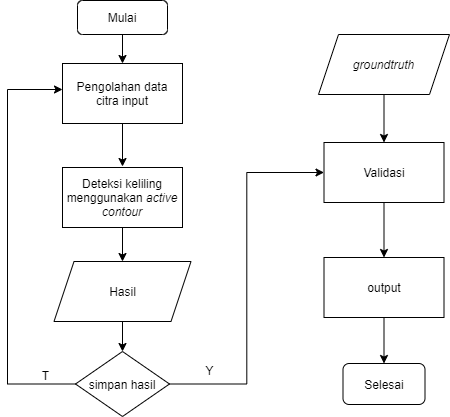
\includegraphics[width=0.6\textwidth]{diagram/metodepenelitian_alur}
	\caption{Diagram alir penelitian}
	\label{Gambar:metodepenelitian_alur}
\end{figure}

\section{Pengolahan data citra input}
Sampel yang baik adalah sampel yang mencerminkan populasinya \citep{amirullah2015metode}. Permata menggunakan data sebanyak 20 citra preparat darah pada penelitiannya tentang segmentasi parasit malaria menggunakan \emph{snake}\citep{permata2015penggunaan}, lalu pada penelitian lain Fadillah menggunakan data sebanyak 15 citra CT-Scan paru-paru pada penelitiannya tentang segmentasi citra paru-paru menggunakan \emph{snake}, dan Constantia menggunakan 21 data citra sapi dalam penelitiannya tentang estimasi bobot sapi menggunakan \emph{snake}\citep{constantia2019estimasi}. 
\begin{comment}
	Tujuan dari sebuah riset adalah untuk memperoleh informasi dari populasi. Populasi merupakan seluruh kumpulan elemen yang dapat digunakan untuk membuat kesimpulan tertentu sedangkan sampel merupakan kelompok yang dipilih dari populasi untuk digunakan dalam riset. Sampai saat ini belum ada kesepakatan atau ketentuan secara ideal dalam menentukan berapa banyak sampel dalam penelitian. 
\end{comment}

% sekaligus sebagai sampel (sampel = populasi), diujikan > tersedia
% mengurangi similarity (luka hitam 1.jpg)
% 28 -> 27 citra, 78 -> 77 citra
\emph{Dataset} luka yang penulis dapat berjumlah 108, sebanyak 37 data tidak dapat dipakai karena data tersebut memiliki duplikasi dengan data lain sehingga data yang tersedia berjumlah 71 buah citra luka yang penulis jadikan sebagai populasi sekaligus sebagai sampel penelitian (sampel = populasi) dengan kategori luka hitam sebanyak 24 citra, luka kuning sebanyak 15 citra, dan luka merah sebanyak 32 citra. \emph{Dataset} ini didapat dari penelitian luka \mbox{Ns. Ratna Aryani, M.Kep}, tahun 2018 \mbox{\citep{ratna2018rancang}} yang tersedia di \emph{repository} \url{https://github.com/mekas/InjuryDetection}. Data yang penulis gunakan adalah data-data yang berekstensi .xcf yang dapat dibuka dengan \emph{software} GIMP, pemrosesan data sebelum deteksi menggunakan \emph{snake} dan GVF dilakukan menggunakan \emph{software} GIMP. \emph{Dataset} ini masing-masing di dalamnya terdapat \emph{layer} citra (luka), \emph{layer} region (luka), dan \emph{path} sebagai berikut :
\begin{figure}[H]
	\centering
	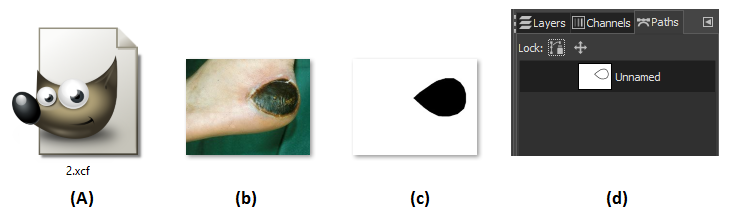
\includegraphics[width=1\textwidth]{gambar/isi_file_xcf}
	\caption{(a) Data citra format .xcf, (b) \emph{layer} citra (luka), (c) \emph{layer} region, (d) \emph{path} }
	\label{Gambar:isi_file_xcf}
\end{figure}

langkah selanjutnya adalah mengubah ukuran (\emph{resize}) citra \emph{size} yang besar ke ukuran yang lebih kecil agar proses deteksi menjadi lebih cepat. Penulis mengubah ukuran citra menggunakan fitur \emph{rescale image} sehingga ukuran citra tidak lebih dari 2 \emph{megabyte}. Kemudian penulis mengecek masing-masing citra dengan fitur \emph{eclipse select} untuk mengetahui apakah objek luka pada data citra pas berada di dalam lingkaran yang akan dijadikan sebagai inisialisasi awal. Ukuran lingkaran tidak boleh lebih besar dari ukuran citra. Jika ukuran lingkaran lebih besar daripada ukuran citra, maka perlu ditambahkan \emph{border} yang dibuat menggunakan fitur \emph{add border} sebagai berikut :
\begin{figure}[H]
	\centering
	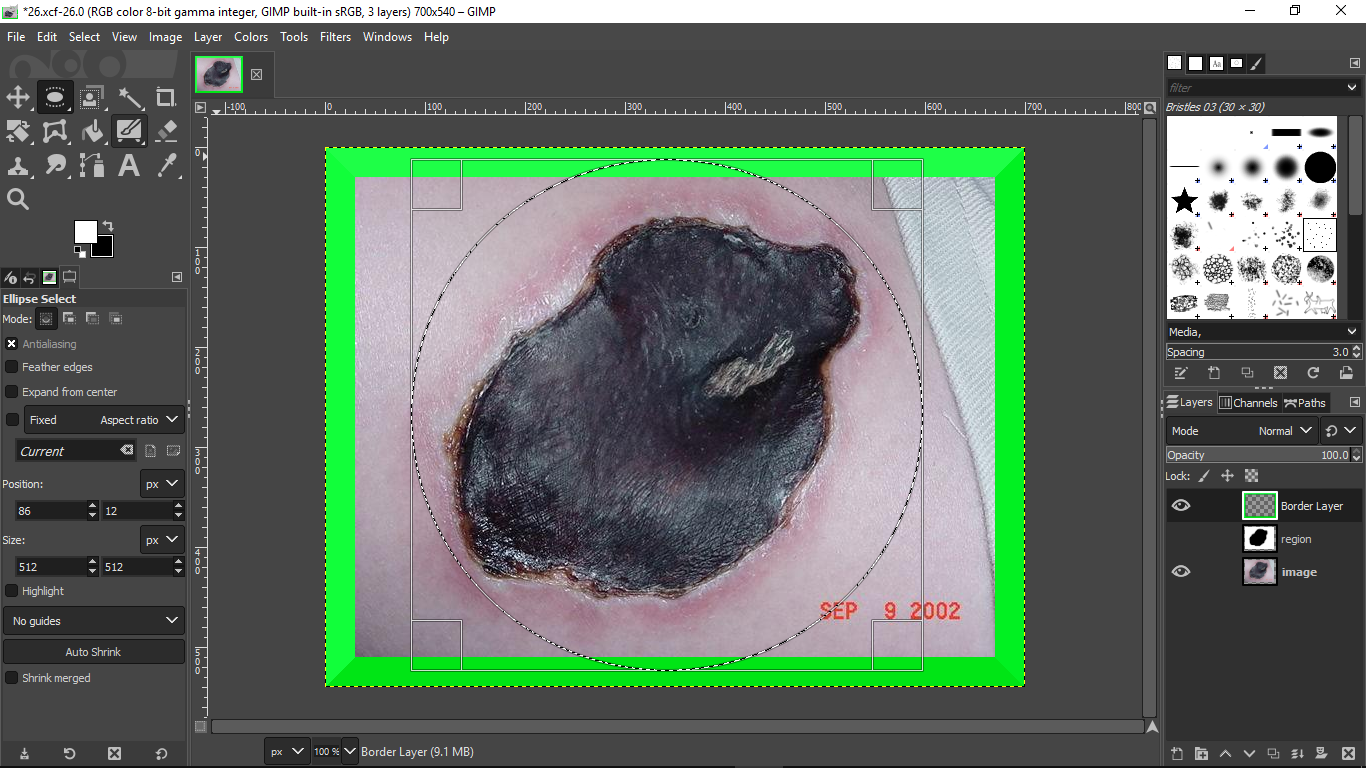
\includegraphics[width=1\textwidth]{gambar/circle_and_border}
	\caption{Citra luka yang telah dicek menggunakan fitur \emph{eclipse select} dan ditambahkan \emph{border}}
	\label{Gambar:circle_and_border}
\end{figure}

Setelah proses \emph{resize} sampai pengecekan lingkaran, selanjutnya penulis \emph{export layer} masing masing ke format .jpg.
\begin{figure}[H]
	\centering
	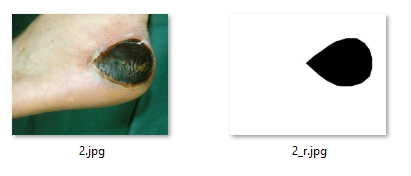
\includegraphics[width=1\textwidth]{gambar/citra_region}
	\caption{Citra luka dan region luka}
	\label{Gambar:citra_region}
\end{figure}




% checkpoint. next olah data di folder my_activecontour

\begin{comment}
\begin{table}[H]
	\centering
	\caption{Rincian data yang akan digunakan kategori luka hitam}
	\label{rinciandataset1}
	\begin{tabular}{|m{1in}|m{1in}|m{1in}|m{1in}|m{1in}|}
		\hline
		\textbf{Citra} & \textbf{\emph{Region}} & \textbf{\emph{Ground truth}} & Kurva awal & Anotasi \\
		\hline
		
		%&  &  & & \\
		%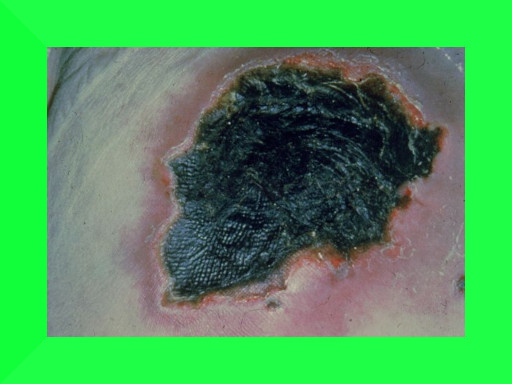
\includegraphics[width=1in]{dataset/dataset_3/luka_hitam/ready/1.jpg} 1.jpg & %
\includegraphics[width=1in]{dataset/dataset_3/luka_hitam/ready/1_r.jpg} 1\_r.jpg & %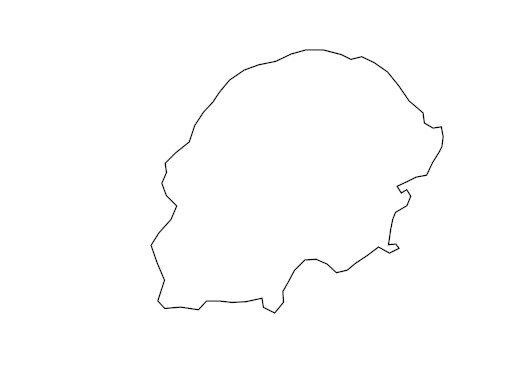
\includegraphics[width=1in]{dataset/dataset_3/luka_hitam/ready/1_g.jpg} 1\_g.jpg &
		%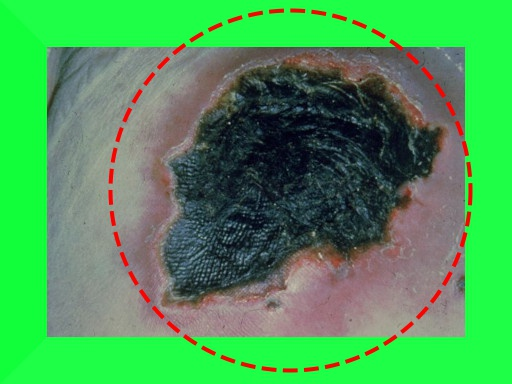
\includegraphics[width=1in]{dataset/dataset_3/luka_hitam/ready/1_init.jpg} 1\_init.jpg &
		%cr=190 
		%cc=290
		%r=180\\
		%\hline
		
		&  &  & & \\
		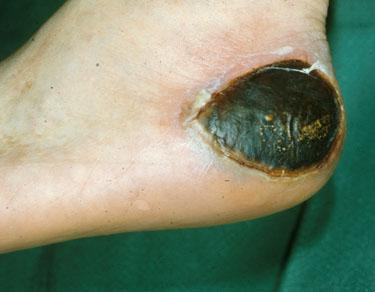
\includegraphics[width=1in]{dataset/dataset_3/luka_hitam/ready/2.jpg} 2.jpg & 
\includegraphics[width=1in]{dataset/dataset_3/luka_hitam/ready/2_r.jpg} 2\_r.jpg & 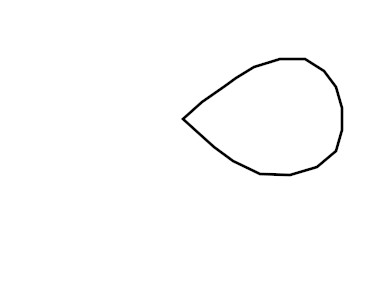
\includegraphics[width=1in]{dataset/dataset_3/luka_hitam/ready/2_g.jpg} 2\_g.jpg &
		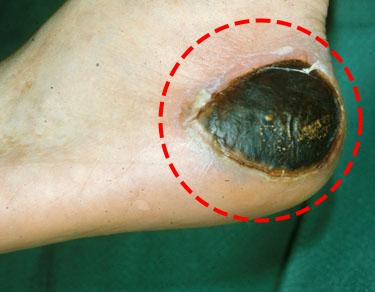
\includegraphics[width=1in]{dataset/dataset_3/luka_hitam/ready/2_init.jpg} 2\_init.jpg &
		cr=120
		cc=265
		r=85\\
		\hline
		
		&  &  & & \\
		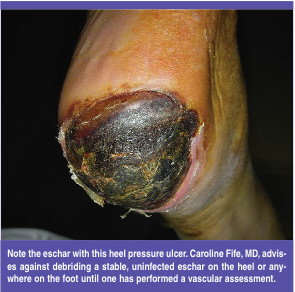
\includegraphics[width=1in]{dataset/dataset_3/luka_hitam/ready/4.jpg} 4.jpg & 
\includegraphics[width=1in]{dataset/dataset_3/luka_hitam/ready/4_r.jpg} 4\_r.jpg & 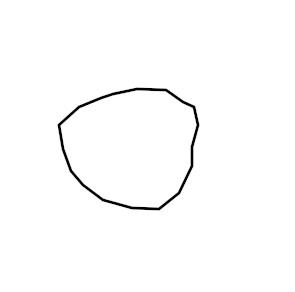
\includegraphics[width=1in]{dataset/dataset_3/luka_hitam/ready/4_g.jpg} 4\_g.jpg &
		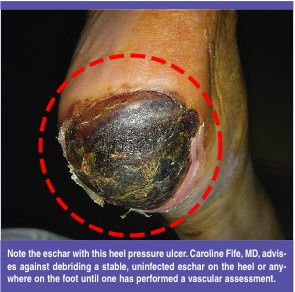
\includegraphics[width=1in]{dataset/dataset_3/luka_hitam/ready/4_init.jpg} 4\_init.jpg &
		cr=145
		cc=130
		r=90\\
		\hline
		
		&  &  & & \\
		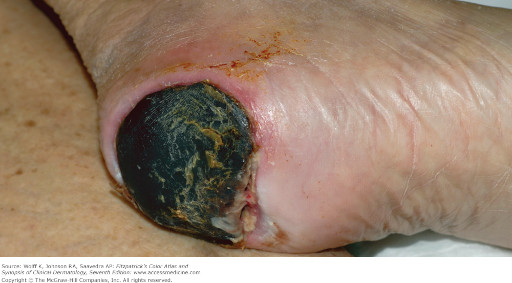
\includegraphics[width=1in]{dataset/dataset_3/luka_hitam/ready/5.jpg} 5.jpg & 
\includegraphics[width=1in]{dataset/dataset_3/luka_hitam/ready/5_r.jpg} 5\_r.jpg & 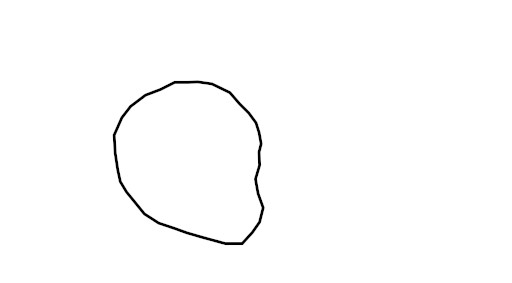
\includegraphics[width=1in]{dataset/dataset_3/luka_hitam/ready/5_g.jpg} 5\_g.jpg &
		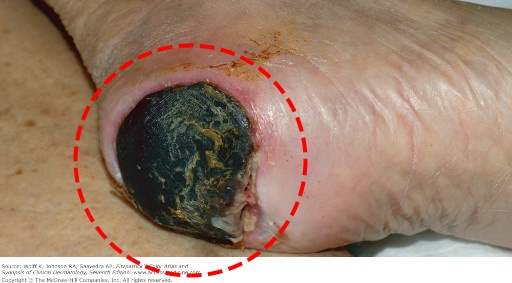
\includegraphics[width=1in]{dataset/dataset_3/luka_hitam/ready/5_init.jpg} 5\_init.jpg &
		cr=160
		cc=190
		r=115\\
		\hline
	\end{tabular}
\end{table}

\begin{table}[H]
	\centering
	\caption{Rincian data yang akan digunakan kategori luka hitam (lanjutan)}
	\label{rinciandataset2}
	\begin{tabular}{|m{1in}|m{1in}|m{1in}|m{1in}|m{1in}|}
		\hline
		\textbf{Citra} & \textbf{\emph{Region}} & \textbf{\emph{Ground truth}} & Kurva awal & Anotasi \\
		\hline
		
		&  &  & & \\
		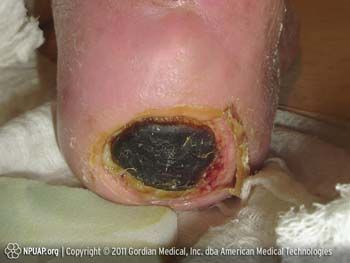
\includegraphics[width=1in]{dataset/dataset_3/luka_hitam/ready/6.jpg} 6.jpg & 
\includegraphics[width=1in]{dataset/dataset_3/luka_hitam/ready/6_r.jpg} 6\_r.jpg & 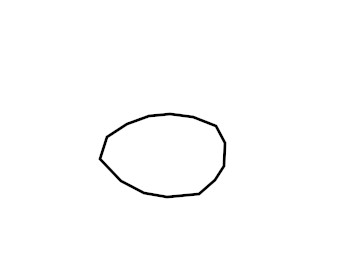
\includegraphics[width=1in]{dataset/dataset_3/luka_hitam/ready/6_g.jpg} 6\_g.jpg &
		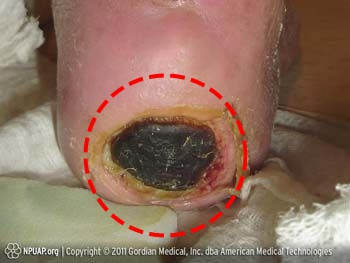
\includegraphics[width=1in]{dataset/dataset_3/luka_hitam/ready/6_init.jpg} 6\_init.jpg &
		cr=155
		cc=165
		r=80\\
		\hline
		
		&  &  & & \\
		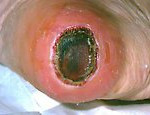
\includegraphics[width=1in]{dataset/dataset_3/luka_hitam/ready/7.jpg} 7.jpg & 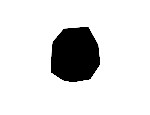
\includegraphics[width=1in]{dataset/dataset_3/luka_hitam/ready/7_r.jpg} 7\_r.jpg & 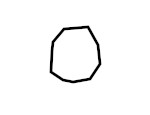
\includegraphics[width=1in]{dataset/dataset_3/luka_hitam/ready/7_g.jpg} 7\_g.jpg &
		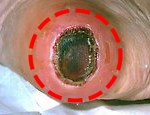
\includegraphics[width=1in]{dataset/dataset_3/luka_hitam/ready/7_init.jpg} 7\_init.jpg &
		cr=55
		cc=75
		r=45\\
		\hline
		
		&  &  & & \\
		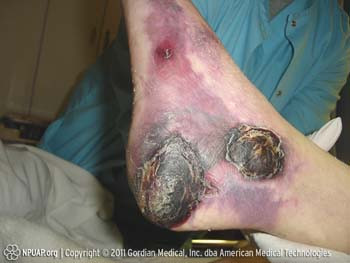
\includegraphics[width=1in]{dataset/dataset_3/luka_hitam/ready/8.jpg} 8.jpg & 
\includegraphics[width=1in]{dataset/dataset_3/luka_hitam/ready/8_r.jpg} 8\_r.jpg & 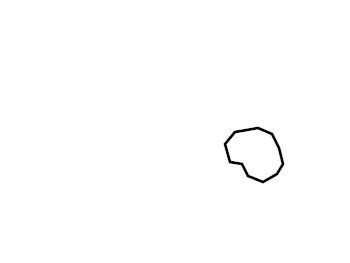
\includegraphics[width=1in]{dataset/dataset_3/luka_hitam/ready/8_g.jpg} 8\_g.jpg &
		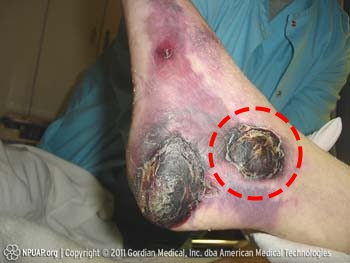
\includegraphics[width=1in]{dataset/dataset_3/luka_hitam/ready/8_init.jpg} 8\_init.jpg &
		cr=153
		cc=255
		r=45\\
		\hline
		
		&  &  & & \\
		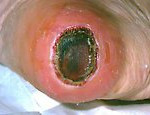
\includegraphics[width=1in]{dataset/dataset_3/luka_hitam/duplicate_or_copyright/9.jpg} 9.jpg & 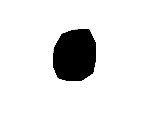
\includegraphics[width=1in]{dataset/dataset_3/luka_hitam/duplicate_or_copyright/9_r.jpg} 9\_r.jpg & 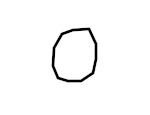
\includegraphics[width=1in]{dataset/dataset_3/luka_hitam/duplicate_or_copyright/9_g.jpg} 9\_g.jpg &
		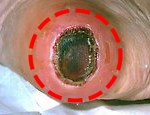
\includegraphics[width=1in]{dataset/dataset_3/luka_hitam/duplicate_or_copyright/9_init.jpg} 9\_init.jpg &
		cr=55
		cc=75
		r=45\\
		\hline
		
		&  &  & & \\
		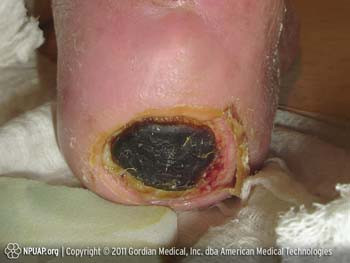
\includegraphics[width=1in]{dataset/dataset_3/luka_hitam/duplicate_or_copyright/11.jpg} 11.jpg & 
\includegraphics[width=1in]{dataset/dataset_3/luka_hitam/duplicate_or_copyright/11_r.jpg} 11\_r.jpg & 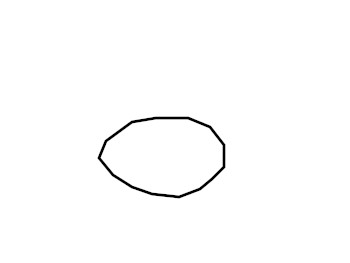
\includegraphics[width=1in]{dataset/dataset_3/luka_hitam/duplicate_or_copyright/11_g.jpg} 11\_g.jpg &
		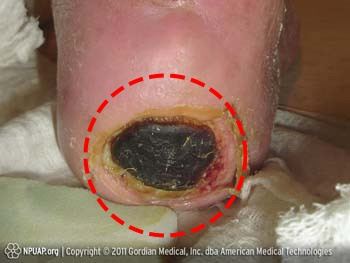
\includegraphics[width=1in]{dataset/dataset_3/luka_hitam/duplicate_or_copyright/11_init.jpg} 11\_init.jpg &
		cr=155
		cc=165
		r=80\\
		\hline
	\end{tabular}
\end{table}

\begin{table}[H]
	\centering
	\caption{Rincian data yang akan digunakan kategori luka hitam (lanjutan)}
	\label{rinciandataset3}
	\begin{tabular}{|m{1in}|m{1in}|m{1in}|m{1in}|m{1in}|}
		\hline
		\textbf{Citra} & \textbf{\emph{Region}} & \textbf{\emph{Ground truth}} & Kurva awal & Anotasi \\
		\hline
		
		&  &  & & \\
		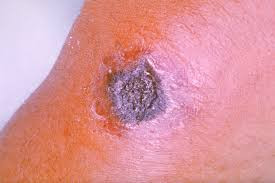
\includegraphics[width=1in]{dataset/dataset_3/luka_hitam/ready/14.jpg} 14.jpg & 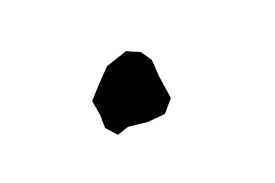
\includegraphics[width=1in]{dataset/dataset_3/luka_hitam/ready/14_r.jpg} 14\_r.jpg & 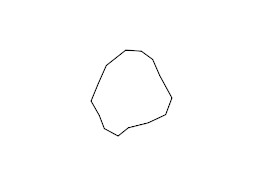
\includegraphics[width=1in]{dataset/dataset_3/luka_hitam/ready/14_g.jpg} 14\_g.jpg &
		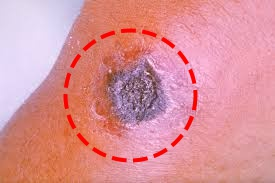
\includegraphics[width=1in]{dataset/dataset_3/luka_hitam/ready/14_init.jpg} 14\_init.jpg &
		cr=95
		cc=130
		r=65\\
		\hline
		
		&  &  & & \\
		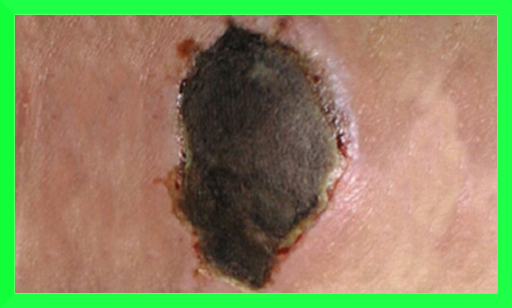
\includegraphics[width=1in]{dataset/dataset_3/luka_hitam/ready/15.jpg} 15.jpg & 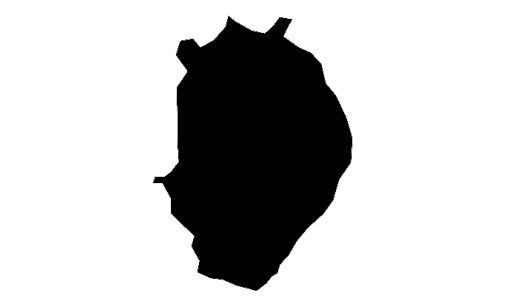
\includegraphics[width=1in]{dataset/dataset_3/luka_hitam/ready/15_r.jpg} 15\_r.jpg & 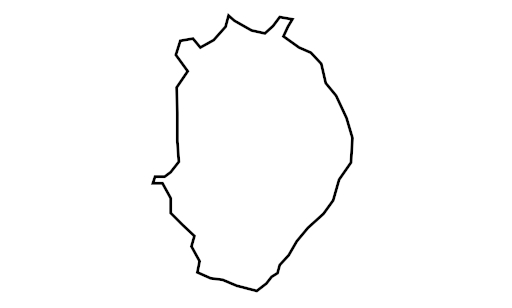
\includegraphics[width=1in]{dataset/dataset_3/luka_hitam/ready/15_g.jpg} 15\_g.jpg &
		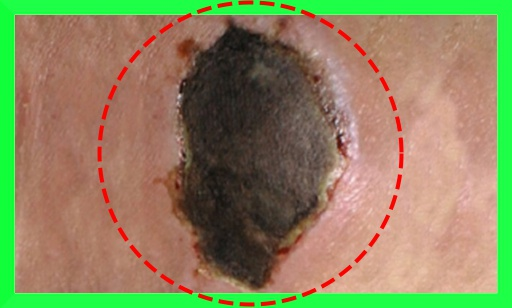
\includegraphics[width=1in]{dataset/dataset_3/luka_hitam/ready/15_init.jpg} 15\_init.jpg &
		cr=153
		cc=250
		r=151\\
		\hline
		
		&  &  & & \\
		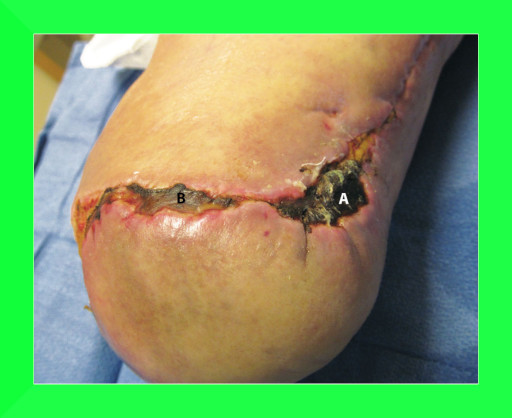
\includegraphics[width=1in]{dataset/dataset_3/luka_hitam/ready/16.jpg} 16.jpg & 
\includegraphics[width=1in]{dataset/dataset_3/luka_hitam/ready/16_r.jpg} 16\_r.jpg & \includegraphics[width=1in]{dataset/dataset_3/luka_hitam/ready/16_g.jpg} 16\_g.jpg &
		\includegraphics[width=1in]{dataset/dataset_3/luka_hitam/ready/16_init.jpg} 16\_init.jpg &
		cr=208
		cc=245
		r=200\\
		\hline
		
		&  &  & & \\
		\includegraphics[width=1in]{dataset/dataset_3/luka_hitam/ready/17.jpg} 17.jpg & \includegraphics[width=1in]{dataset/dataset_3/luka_hitam/ready/17_r.jpg} 17\_r.jpg & \includegraphics[width=1in]{dataset/dataset_3/luka_hitam/ready/17_g.jpg} 17\_g.jpg &
		\includegraphics[width=1in]{dataset/dataset_3/luka_hitam/ready/17_init.jpg} 17\_init.jpg &
		cr=124
		cc=125
		r=120\\
		\hline
		
		&  &  & & \\
		\includegraphics[width=1in]{dataset/dataset_3/luka_hitam/ready/18.jpg} 18.jpg & \includegraphics[width=1in]{dataset/dataset_3/luka_hitam/ready/18_r.jpg} 18\_r.jpg & \includegraphics[width=1in]{dataset/dataset_3/luka_hitam/ready/18_g.jpg} 18\_g.jpg &
		\includegraphics[width=1in]{dataset/dataset_3/luka_hitam/ready/18_init.jpg} 18\_init.jpg &
		cr=85
		cc=85
		r=75\\
		\hline
	\end{tabular}
\end{table}

\begin{table}[H]
	\centering
	\caption{Rincian data yang akan digunakan kategori luka hitam (lanjutan)}
	\label{rinciandataset4}
	\begin{tabular}{|m{1in}|m{1in}|m{1in}|m{1in}|m{1in}|}
		\hline
		\textbf{Citra} & \textbf{\emph{Region}} & \textbf{\emph{Ground truth}} & Kurva awal & Anotasi \\
		\hline
		
		&  &  & & \\
		\includegraphics[width=1in]{dataset/dataset_3/luka_hitam/ready/19.jpg} 19.jpg & \includegraphics[width=1in]{dataset/dataset_3/luka_hitam/ready/19_r.jpg} 19\_r.jpg & \includegraphics[width=1in]{dataset/dataset_3/luka_hitam/ready/19_g.jpg} 19\_g.jpg &
		\includegraphics[width=1in]{dataset/dataset_3/luka_hitam/ready/19_init.jpg} 19\_init.jpg &
		cr=225
		cc=285
		r=130\\
		\hline
		
		&  &  & & \\
		\includegraphics[width=1in]{dataset/dataset_3/luka_hitam/ready/20.jpg} 20.jpg & \includegraphics[width=1in]{dataset/dataset_3/luka_hitam/ready/20_r.jpg} 20\_r.jpg & \includegraphics[width=1in]{dataset/dataset_3/luka_hitam/ready/20_g.jpg} 20\_g.jpg &
		\includegraphics[width=1in]{dataset/dataset_3/luka_hitam/ready/20_init.jpg} 20\_init.jpg &
		cr=250
		cc=225
		r=155\\
		\hline
		
		&  &  & & \\
		\includegraphics[width=1in]{dataset/dataset_3/luka_hitam/ready/22.jpg} 22.jpg & \includegraphics[width=1in]{dataset/dataset_3/luka_hitam/ready/22_r.jpg} 22\_r.jpg & \includegraphics[width=1in]{dataset/dataset_3/luka_hitam/ready/22_g.jpg} 22\_g.jpg &
		\includegraphics[width=1in]{dataset/dataset_3/luka_hitam/ready/22_init.jpg} 22\_init.jpg &
		cr=140
		cc=190
		r=125\\
		\hline
		
		&  &  & & \\
		\includegraphics[width=1in]{dataset/dataset_3/luka_hitam/duplicate_or_copyright/24.jpg} 24.jpg & \includegraphics[width=1in]{dataset/dataset_3/luka_hitam/duplicate_or_copyright/24_r.jpg} 24\_r.jpg & \includegraphics[width=1in]{dataset/dataset_3/luka_hitam/duplicate_or_copyright/24_g.jpg} 24\_g.jpg &
		\includegraphics[width=1in]{dataset/dataset_3/luka_hitam/duplicate_or_copyright/24_init.jpg} 24\_init.jpg &
		cr=190
		cc=190
		r=180\\
		\hline
		
		&  &  & & \\
		\includegraphics[width=1in]{dataset/dataset_3/luka_hitam/ready/26.jpg} 26.jpg & \includegraphics[width=1in]{dataset/dataset_3/luka_hitam/ready/26_r.jpg} 26\_r.jpg & \includegraphics[width=1in]{dataset/dataset_3/luka_hitam/ready/26_g.jpg} 26\_g.jpg &
		\includegraphics[width=1in]{dataset/dataset_3/luka_hitam/ready/26_init.jpg} 26\_init.jpg &
		cr=195
		cc=248
		r=193\\
		\hline
	\end{tabular}
\end{table}

\begin{table}[H]
	\centering
	\caption{Rincian data yang akan digunakan kategori luka hitam (lanjutan)}
	\label{rinciandataset5}
	\begin{tabular}{|m{1in}|m{1in}|m{1in}|m{1in}|m{1in}|}
		\hline
		\textbf{Citra} & \textbf{\emph{Region}} & \textbf{\emph{Ground truth}} & Kurva awal & Anotasi \\
		\hline
		
		&  &  & & \\
		\includegraphics[width=1in]{dataset/dataset_3/luka_hitam/ready/27.jpg} 27.jpg & \includegraphics[width=1in]{dataset/dataset_3/luka_hitam/ready/27_r.jpg} 27\_r.jpg & \includegraphics[width=1in]{dataset/dataset_3/luka_hitam/ready/27_g.jpg} 27\_g.jpg &
		\includegraphics[width=1in]{dataset/dataset_3/luka_hitam/ready/27_init.jpg} 27\_init.jpg &
		cr=207
		cc=253
		r=205\\
		\hline
		
		&  &  & & \\
		\includegraphics[width=1in]{dataset/dataset_3/luka_hitam/ready/28.jpg} 28.jpg & \includegraphics[width=1in]{dataset/dataset_3/luka_hitam/ready/28_r.jpg} 28\_r.jpg & \includegraphics[width=1in]{dataset/dataset_3/luka_hitam/ready/28_g.jpg} 28\_g.jpg &
		\includegraphics[width=1in]{dataset/dataset_3/luka_hitam/ready/28_init.jpg} 28\_init.jpg &
		cr=120
		cc=80
		r=70\\
		\hline
		
		&  &  & & \\
		\includegraphics[width=1in]{dataset/dataset_3/luka_hitam/ready/29.jpg} 29.jpg & \includegraphics[width=1in]{dataset/dataset_3/luka_hitam/ready/29_r.jpg} 29\_r.jpg & \includegraphics[width=1in]{dataset/dataset_3/luka_hitam/ready/29_g.jpg} 29\_g.jpg &
		\includegraphics[width=1in]{dataset/dataset_3/luka_hitam/ready/16_init.jpg} 29\_init.jpg &
		cr=195
		cc=240
		r=180\\
		\hline
		
		&  &  & & \\
		\includegraphics[width=1in]{dataset/dataset_3/luka_hitam/ready/31.jpg} 31.jpg & \includegraphics[width=1in]{dataset/dataset_3/luka_hitam/ready/31_r.jpg} 31\_r.jpg & \includegraphics[width=1in]{dataset/dataset_3/luka_hitam/ready/31_g.jpg} 31\_g.jpg &
		\includegraphics[width=1in]{dataset/dataset_3/luka_hitam/ready/31_init.jpg} 31\_init.jpg &
		cr=245
		cc=190
		r=180\\
		\hline
		
		&  &  & & \\
		\includegraphics[width=1in]{dataset/dataset_3/luka_hitam/ready/33.jpg} 33.jpg & \includegraphics[width=1in]{dataset/dataset_3/luka_hitam/ready/33_r.jpg} 33\_r.jpg & \includegraphics[width=1in]{dataset/dataset_3/luka_hitam/ready/33_g.jpg} 33\_g.jpg &
		\includegraphics[width=1in]{dataset/dataset_3/luka_hitam/ready/33_init.jpg} 33\_init.jpg &
		cr=120
		cc=195
		r=100\\
		\hline
	\end{tabular}
\end{table}

\begin{table}[H]
	\centering
	\caption{Rincian data yang akan digunakan kategori luka hitam (lanjutan)}
	\label{rinciandataset6}
	\begin{tabular}{|m{1in}|m{1in}|m{1in}|m{1in}|m{1in}|}
		\hline
		\textbf{Citra} & \textbf{\emph{Region}} & \textbf{\emph{Ground truth}} & Kurva awal & Anotasi \\
		\hline
		
		&  &  & & \\
		\includegraphics[width=1in]{dataset/dataset_3/luka_hitam/ready/37.jpg} 37.jpg & \includegraphics[width=1in]{dataset/dataset_3/luka_hitam/ready/37_r.jpg} 37\_r.jpg & \includegraphics[width=1in]{dataset/dataset_3/luka_hitam/ready/37_g.jpg} 37\_g.jpg &
		\includegraphics[width=1in]{dataset/dataset_3/luka_hitam/ready/37_init.jpg} 37\_init.jpg &
		cr=110
		cc=125
		r=95\\
		\hline
		
		&  &  & & \\
		\includegraphics[width=1in]{dataset/dataset_3/luka_hitam/ready/39.jpg} 39.jpg & \includegraphics[width=1in]{dataset/dataset_3/luka_hitam/ready/39_r.jpg} 39\_r.jpg & \includegraphics[width=1in]{dataset/dataset_3/luka_hitam/ready/39_g.jpg} 39\_g.jpg &
		\includegraphics[width=1in]{dataset/dataset_3/luka_hitam/ready/39_init.jpg} 39\_init.jpg &
		cr=260
		cc=265
		r=170\\
		\hline
		
		&  &  & & \\
		\includegraphics[width=1in]{dataset/dataset_3/luka_hitam/ready/40.jpg} 40.jpg & \includegraphics[width=1in]{dataset/dataset_3/luka_hitam/ready/40_r.jpg} 40\_r.jpg & \includegraphics[width=1in]{dataset/dataset_3/luka_hitam/ready/40_g.jpg} 40\_g.jpg &
		\includegraphics[width=1in]{dataset/dataset_3/luka_hitam/ready/40_init.jpg} 40\_init.jpg &
		cr=90
		cc=100
		r=65\\
		\hline
		
		&  &  & & \\
		\includegraphics[width=1in]{dataset/dataset_3/luka_hitam/ready/41.jpg} 41.jpg & \includegraphics[width=1in]{dataset/dataset_3/luka_hitam/ready/41_r.jpg} 41\_r.jpg & \includegraphics[width=1in]{dataset/dataset_3/luka_hitam/ready/41_g.jpg} 41\_g.jpg &
		\includegraphics[width=1in]{dataset/dataset_3/luka_hitam/ready/41_init.jpg} 41\_init.jpg &
		cr=105
		cc=170
		r=100\\
		\hline
	\end{tabular}
\end{table}


\begin{table}[H]
	\centering
	\caption{Rincian data yang akan digunakan kategori luka kuning}
	\label{rinciandataset7}
	\begin{tabular}{|m{1in}|m{1in}|m{1in}|m{1in}|m{1in}|}
		\hline
		\textbf{Citra} & \textbf{\emph{Region}} & \textbf{\emph{Ground truth}} & Kurva awal & Anotasi \\
		\hline
		
		&  &  & & \\
		\includegraphics[width=1in]{dataset/dataset_3/luka_kuning/ready/3.jpg} 3.jpg & \includegraphics[width=1in]{dataset/dataset_3/luka_kuning/ready/3_r.jpg} 3\_r.jpg & \includegraphics[width=1in]{dataset/dataset_3/luka_kuning/ready/3_g.jpg} 3\_g.jpg &
		\includegraphics[width=1in]{dataset/dataset_3/luka_kuning/ready/3_init.jpg} 3\_init.jpg &
		cr=80
		cc=85
		r=65\\
		\hline
		
		&  &  & & \\
		\includegraphics[width=1in]{dataset/dataset_3/luka_kuning/ready/10.jpg} 10.jpg & \includegraphics[width=1in]{dataset/dataset_3/luka_kuning/ready/10_r.jpg} 10\_r.jpg & \includegraphics[width=1in]{dataset/dataset_3/luka_kuning/ready/10_g.jpg} 10\_g.jpg &
		\includegraphics[width=1in]{dataset/dataset_3/luka_kuning/ready/10_init.jpg} 10\_init.jpg &
		cr=155
		cc=133
		r=128\\
		\hline
		
		&  &  & & \\
		\includegraphics[width=1in]{dataset/dataset_3/luka_kuning/ready/12.jpg} 12.jpg & \includegraphics[width=1in]{dataset/dataset_3/luka_kuning/ready/12_r.jpg} 12\_r.jpg & \includegraphics[width=1in]{dataset/dataset_3/luka_kuning/ready/12_g.jpg} 12\_g.jpg &
		\includegraphics[width=1in]{dataset/dataset_3/luka_kuning/ready/12_init.jpg} 12\_init.jpg &
		cr=90
		cc=138
		r=70\\
		\hline
		
		&  &  & & \\
		\includegraphics[width=1in]{dataset/dataset_3/luka_kuning/ready/13.jpg} 13.jpg & \includegraphics[width=1in]{dataset/dataset_3/luka_kuning/ready/13_r.jpg} 13\_r.jpg & \includegraphics[width=1in]{dataset/dataset_3/luka_kuning/ready/13_g.jpg} 13\_g.jpg &
		\includegraphics[width=1in]{dataset/dataset_3/luka_kuning/ready/13_init.jpg} 13\_init.jpg &
		cr=70
		cc=206
		r=50\\
		\hline
		
		&  &  & & \\
		\includegraphics[width=1in]{dataset/dataset_3/luka_kuning/ready/16.jpg} 16.jpg & \includegraphics[width=1in]{dataset/dataset_3/luka_kuning/ready/16_r.jpg} 16\_r.jpg & \includegraphics[width=1in]{dataset/dataset_3/luka_kuning/ready/16_g.jpg} 16\_g.jpg &
		\includegraphics[width=1in]{dataset/dataset_3/luka_kuning/ready/16_init.jpg} 16\_init.jpg &
		cr=135
		cc=172
		r=130\\
		\hline
	\end{tabular}
\end{table}

\begin{table}[H]
	\centering
	\caption{Rincian data yang akan digunakan kategori luka kuning (lanjutan)}
	\label{rinciandataset8}
	\begin{tabular}{|m{1in}|m{1in}|m{1in}|m{1in}|m{1in}|}
		\hline
		\textbf{Citra} & \textbf{\emph{Region}} & \textbf{\emph{Ground truth}} & Kurva awal & Anotasi \\
		\hline
		
		&  &  & & \\
		\includegraphics[width=1in]{dataset/dataset_3/luka_kuning/ready/17.jpg} 17.jpg & \includegraphics[width=1in]{dataset/dataset_3/luka_kuning/ready/17_r.jpg} 17\_r.jpg & \includegraphics[width=1in]{dataset/dataset_3/luka_kuning/ready/17_g.jpg} 17\_g.jpg &
		\includegraphics[width=1in]{dataset/dataset_3/luka_kuning/ready/17_init.jpg} 17\_init.jpg &
		cr=125
		cc=115
		r=25\\
		\hline
		
		&  &  & & \\
		\includegraphics[width=1in]{dataset/dataset_3/luka_kuning/ready/18.jpg} 18.jpg & \includegraphics[width=1in]{dataset/dataset_3/luka_kuning/ready/18_r.jpg} 18\_r.jpg & \includegraphics[width=1in]{dataset/dataset_3/luka_kuning/ready/18_g.jpg} 18\_g.jpg &
		\includegraphics[width=1in]{dataset/dataset_3/luka_kuning/ready/18_init.jpg} 18\_init.jpg &
		cr=95
		cc=130
		r=80\\
		\hline
		
		&  &  & & \\
		\includegraphics[width=1in]{dataset/dataset_3/luka_kuning/ready/19.jpg} 19.jpg & \includegraphics[width=1in]{dataset/dataset_3/luka_kuning/ready/19_r.jpg} 19\_r.jpg & \includegraphics[width=1in]{dataset/dataset_3/luka_kuning/ready/19_g.jpg} 19\_g.jpg &
		\includegraphics[width=1in]{dataset/dataset_3/luka_kuning/ready/19_init.jpg} 19\_init.jpg &
		cr=60
		cc=60
		r=50\\
		\hline
		
		&  &  & & \\
		\includegraphics[width=1in]{dataset/dataset_3/luka_kuning/ready/21.jpg} 21.jpg & \includegraphics[width=1in]{dataset/dataset_3/luka_kuning/ready/21_r.jpg} 21\_r.jpg & \includegraphics[width=1in]{dataset/dataset_3/luka_kuning/ready/21_g.jpg} 21\_g.jpg &
		\includegraphics[width=1in]{dataset/dataset_3/luka_kuning/ready/21_init.jpg} 21\_init.jpg &
		cr=130
		cc=170
		r=70\\
		\hline
		
		&  &  & & \\
		\includegraphics[width=1in]{dataset/dataset_3/luka_kuning/ready/23.jpg} 23.jpg & \includegraphics[width=1in]{dataset/dataset_3/luka_kuning/ready/23_r.jpg} 23\_r.jpg & \includegraphics[width=1in]{dataset/dataset_3/luka_kuning/ready/23_g.jpg} 23\_g.jpg &
		\includegraphics[width=1in]{dataset/dataset_3/luka_kuning/ready/23_init.jpg} 23\_init.jpg &
		cr=170
		cc=230
		r=160\\
		\hline
	\end{tabular}
\end{table}

\begin{table}[H]
	\centering
	\caption{Rincian data yang akan digunakan kategori luka kuning (lanjutan)}
	\label{rinciandataset9}
	\begin{tabular}{|m{1in}|m{1in}|m{1in}|m{1in}|m{1in}|}
		\hline
		\textbf{Citra} & \textbf{\emph{Region}} & \textbf{\emph{Ground truth}} & Kurva awal & Anotasi \\
		\hline
		
		&  &  & & \\
		\includegraphics[width=1in]{dataset/dataset_3/luka_kuning/ready/25.jpg} 25.jpg & \includegraphics[width=1in]{dataset/dataset_3/luka_kuning/ready/25_r.jpg} 25\_r.jpg & \includegraphics[width=1in]{dataset/dataset_3/luka_kuning/ready/25_g.jpg} 25\_g.jpg &
		\includegraphics[width=1in]{dataset/dataset_3/luka_kuning/ready/25_init.jpg} 25\_init.jpg &
		cr=145
		cc=130
		r=55\\
		\hline
		
		&  &  & & \\
		\includegraphics[width=1in]{dataset/dataset_3/luka_kuning/ready/34.jpg} 34.jpg & \includegraphics[width=1in]{dataset/dataset_3/luka_kuning/ready/34_r.jpg} 34\_r.jpg & \includegraphics[width=1in]{dataset/dataset_3/luka_kuning/ready/34_g.jpg} 34\_g.jpg &
		\includegraphics[width=1in]{dataset/dataset_3/luka_kuning/ready/34_init.jpg} 34\_init.jpg &
		cr=185
		cc=245
		r=130\\
		\hline
		
		&  &  & & \\
		\includegraphics[width=1in]{dataset/dataset_3/luka_kuning/ready/35.jpg} 35.jpg & \includegraphics[width=1in]{dataset/dataset_3/luka_kuning/ready/35_r.jpg} 35\_r.jpg & \includegraphics[width=1in]{dataset/dataset_3/luka_kuning/ready/35_g.jpg} 35\_g.jpg &
		\includegraphics[width=1in]{dataset/dataset_3/luka_kuning/ready/35_init.jpg} 35\_init.jpg &
		cr=105
		cc=110
		r=100\\
		\hline
		
		&  &  & & \\
		\includegraphics[width=1in]{dataset/dataset_3/luka_kuning/ready/38.jpg} 38.jpg & \includegraphics[width=1in]{dataset/dataset_3/luka_kuning/ready/38_r.jpg} 38\_r.jpg & \includegraphics[width=1in]{dataset/dataset_3/luka_kuning/ready/38_g.jpg} 38\_g.jpg &
		\includegraphics[width=1in]{dataset/dataset_3/luka_kuning/ready/38_init.jpg} 38\_init.jpg &
		cr=150
		cc=280
		r=120\\
		\hline
		
		&  &  & & \\
		\includegraphics[width=1in]{dataset/dataset_3/luka_kuning/ready/42.jpg} 42.jpg & \includegraphics[width=1in]{dataset/dataset_3/luka_kuning/ready/42_r.jpg} 42\_r.jpg & \includegraphics[width=1in]{dataset/dataset_3/luka_kuning/ready/42_g.jpg} 42\_g.jpg &
		\includegraphics[width=1in]{dataset/dataset_3/luka_kuning/ready/42_init.jpg} 42\_init.jpg &
		cr=160
		cc=260
		r=1135\\
		\hline
	\end{tabular}
\end{table}


\begin{table}[H]
	\centering
	\caption{Rincian data yang akan digunakan kategori luka merah }
	\label{rinciandataset10}
	\begin{tabular}{|m{1in}|m{1in}|m{1in}|m{1in}|m{1in}|}
		\hline
		\textbf{Citra} & \textbf{\emph{Region}} & \textbf{\emph{Ground truth}} & Kurva awal & Anotasi \\
		\hline
		
		&  &  & & \\
		\includegraphics[width=0.8in]{dataset/dataset_3/luka_merah/ready/1.jpg} 1.jpg & \includegraphics[width=0.8in]{dataset/dataset_3/luka_merah/ready/1_r.jpg} 1\_r.jpg & \includegraphics[width=0.8in]{dataset/dataset_3/luka_merah/ready/1_g.jpg} 1\_g.jpg &
		\includegraphics[width=0.8in]{dataset/dataset_3/luka_merah/ready/1_init.jpg} 1\_init.jpg &
		cr=200
		cc=235
		r=190\\
		\hline
		
		&  &  & & \\
		\includegraphics[width=0.8in]{dataset/dataset_3/luka_merah/ready/2.jpg} 2.jpg & \includegraphics[width=0.8in]{dataset/dataset_3/luka_merah/ready/2_r.jpg} 2\_r.jpg & \includegraphics[width=0.8in]{dataset/dataset_3/luka_merah/ready/2_g.jpg} 2\_g.jpg &
		\includegraphics[width=0.8in]{dataset/dataset_3/luka_merah/ready/2_init.jpg} 2\_init.jpg &
		cr=270
		cc=105
		r=100\\
		\hline
		
		&  &  & & \\
		\includegraphics[width=0.8in]{dataset/dataset_3/luka_merah/ready/3.jpg} 3.jpg & \includegraphics[width=0.8in]{dataset/dataset_3/luka_merah/ready/3_r.jpg} 3\_r.jpg & \includegraphics[width=0.8in]{dataset/dataset_3/luka_merah/ready/3_g.jpg} 3\_g.jpg &
		\includegraphics[width=0.8in]{dataset/dataset_3/luka_merah/ready/3_init.jpg} 3\_init.jpg &
		cr=255
		cc=170
		r=100\\
		\hline
		
		&  &  & & \\
		\includegraphics[width=0.8in]{dataset/dataset_3/luka_merah/ready/4.jpg} 4.jpg & \includegraphics[width=0.8in]{dataset/dataset_3/luka_merah/ready/4_r.jpg} 4\_r.jpg & \includegraphics[width=0.8in]{dataset/dataset_3/luka_merah/ready/4_g.jpg} 4\_g.jpg &
		\includegraphics[width=0.8in]{dataset/dataset_3/luka_merah/ready/4_init.jpg} 4\_init.jpg &
		cr=310
		cc=170
		r=150\\
		\hline
		
		&  &  & & \\
		\includegraphics[width=0.8in]{dataset/dataset_3/luka_merah/ready/6.jpg} 6.jpg & \includegraphics[width=0.8in]{dataset/dataset_3/luka_merah/ready/6_r.jpg} 6\_r.jpg & \includegraphics[width=0.8in]{dataset/dataset_3/luka_merah/ready/6_g.jpg} 6\_g.jpg &
		\includegraphics[width=0.8in]{dataset/dataset_3/luka_merah/ready/6_init.jpg} 6\_init.jpg &
		cr=160
		cc=250
		r=120\\
		\hline
	\end{tabular}
\end{table}

\begin{table}[H]
	\centering
	\caption{Rincian data yang akan digunakan kategori luka merah (lanjutan)}
	\label{rinciandataset11}
	\begin{tabular}{|m{1in}|m{1in}|m{1in}|m{1in}|m{1in}|}
		\hline
		\textbf{Citra} & \textbf{\emph{Region}} & \textbf{\emph{Ground truth}} & Kurva awal & Anotasi \\
		\hline
		
		&  &  & & \\
		\includegraphics[width=1in]{dataset/dataset_3/luka_merah/ready/7.jpg} 7.jpg & \includegraphics[width=1in]{dataset/dataset_3/luka_merah/ready/7_r.jpg} 7\_r.jpg & \includegraphics[width=1in]{dataset/dataset_3/luka_merah/ready/7_g.jpg} 7\_g.jpg &
		\includegraphics[width=1in]{dataset/dataset_3/luka_merah/ready/7_init.jpg} 7\_init.jpg &
		cr=180
		cc=250
		r=90\\
		\hline
		
		&  &  & & \\
		\includegraphics[width=1in]{dataset/dataset_3/luka_merah/ready/8.jpg} 8.jpg & \includegraphics[width=1in]{dataset/dataset_3/luka_merah/ready/8_r.jpg} 8\_r.jpg & \includegraphics[width=1in]{dataset/dataset_3/luka_merah/ready/8_g.jpg} 8\_g.jpg &
		\includegraphics[width=1in]{dataset/dataset_3/luka_merah/ready/8_init.jpg} 8\_init.jpg &
		cr=220
		cc=260
		r=140\\
		\hline
		
		&  &  & & \\
		\includegraphics[width=1in]{dataset/dataset_3/luka_merah/ready/9.jpg} 9.jpg & \includegraphics[width=1in]{dataset/dataset_3/luka_merah/ready/9_r.jpg} 9\_r.jpg & \includegraphics[width=1in]{dataset/dataset_3/luka_merah/ready/9_g.jpg} 9\_g.jpg &
		\includegraphics[width=1in]{dataset/dataset_3/luka_merah/ready/9_init.jpg} 9\_init.jpg &
		cr=236
		cc=130
		r=70\\
		\hline
		
		&  &  & & \\
		\includegraphics[width=1in]{dataset/dataset_3/luka_merah/ready/10.jpg} 10.jpg & \includegraphics[width=1in]{dataset/dataset_3/luka_merah/ready/10_r.jpg} 10\_r.jpg & \includegraphics[width=1in]{dataset/dataset_3/luka_merah/ready/10_g.jpg} 10\_g.jpg &
		\includegraphics[width=1in]{dataset/dataset_3/luka_merah/ready/10_init.jpg} 10\_init.jpg &
		cr=180
		cc=240
		r=90\\
		\hline
		
		&  &  & & \\
		\includegraphics[width=1in]{dataset/dataset_3/luka_merah/ready/11.jpg} 11.jpg & \includegraphics[width=1in]{dataset/dataset_3/luka_merah/ready/11_r.jpg} 11\_r.jpg & \includegraphics[width=1in]{dataset/dataset_3/luka_merah/ready/11_g.jpg} 11\_g.jpg &
		\includegraphics[width=1in]{dataset/dataset_3/luka_merah/ready/11_init.jpg} 11\_init.jpg &
		cr=190
		cc=295
		r=170\\
		\hline
	\end{tabular}
\end{table}

\begin{table}[H]
	\centering
	\caption{Rincian data yang akan digunakan kategori luka merah (lanjutan)}
	\label{rinciandataset12}
	\begin{tabular}{|m{1in}|m{1in}|m{1in}|m{1in}|m{1in}|}
		\hline
		\textbf{Citra} & \textbf{\emph{Region}} & \textbf{\emph{Ground truth}} & Kurva awal & Anotasi \\
		\hline
		
		&  &  & & \\
		\includegraphics[width=1in]{dataset/dataset_3/luka_merah/ready/12.jpg} 12.jpg & \includegraphics[width=1in]{dataset/dataset_3/luka_merah/ready/12_r.jpg} 12\_r.jpg & \includegraphics[width=1in]{dataset/dataset_3/luka_merah/ready/12_g.jpg} 12\_g.jpg &
		\includegraphics[width=1in]{dataset/dataset_3/luka_merah/ready/12_init.jpg} 12\_init.jpg &
		cr=200
		cc=245
		r=155\\
		\hline
		
		&  &  & & \\
		\includegraphics[width=1in]{dataset/dataset_3/luka_merah/ready/14.jpg} 14.jpg & \includegraphics[width=1in]{dataset/dataset_3/luka_merah/ready/14_r.jpg} 14\_r.jpg & \includegraphics[width=1in]{dataset/dataset_3/luka_merah/ready/14_g.jpg} 14\_g.jpg &
		\includegraphics[width=1in]{dataset/dataset_3/luka_merah/ready/14_init.jpg} 14\_init.jpg &
		cr=180
		cc=263
		r=175\\
		\hline
		
		&  &  & & \\
		\includegraphics[width=1in]{dataset/dataset_3/luka_merah/ready/16.jpg} 16.jpg & \includegraphics[width=1in]{dataset/dataset_3/luka_merah/ready/16_r.jpg} 16\_r.jpg & \includegraphics[width=1in]{dataset/dataset_3/luka_merah/ready/16_g.jpg} 16\_g.jpg &
		\includegraphics[width=1in]{dataset/dataset_3/luka_merah/ready/16_init.jpg} 16\_init.jpg &
		cr=105
		cc=140
		r=90\\
		\hline
		
		&  &  & & \\
		\includegraphics[width=1in]{dataset/dataset_3/luka_merah/ready/17.jpg} 17.jpg & \includegraphics[width=1in]{dataset/dataset_3/luka_merah/ready/17_r.jpg} 17\_r.jpg & \includegraphics[width=1in]{dataset/dataset_3/luka_merah/ready/17_g.jpg} 17\_g.jpg &
		\includegraphics[width=1in]{dataset/dataset_3/luka_merah/ready/17_init.jpg} 17\_init.jpg &
		cr=105
		cc=160
		r=90\\
		\hline
		
		&  &  & & \\
		\includegraphics[width=1in]{dataset/dataset_3/luka_merah/ready/18.jpg} 18.jpg & \includegraphics[width=1in]{dataset/dataset_3/luka_merah/ready/18_r.jpg} 18\_r.jpg & \includegraphics[width=1in]{dataset/dataset_3/luka_merah/ready/18_g.jpg} 18\_g.jpg &
		\includegraphics[width=1in]{dataset/dataset_3/luka_merah/ready/18_init.jpg} 18\_init.jpg &
		cr=180
		cc=280
		r=70\\
		\hline
	\end{tabular}
\end{table}

\begin{table}[H]
	\centering
	\caption{Rincian data yang akan digunakan kategori luka merah (lanjutan) }
	\label{rinciandataset13}
	\begin{tabular}{|m{1in}|m{1in}|m{1in}|m{1in}|m{1in}|}
		\hline
		\textbf{Citra} & \textbf{\emph{Region}} & \textbf{\emph{Ground truth}} & Kurva awal & Anotasi \\
		\hline
		
		&  &  & & \\
		\includegraphics[width=1in]{dataset/dataset_3/luka_merah/ready/19.jpg} 19.jpg & \includegraphics[width=1in]{dataset/dataset_3/luka_merah/ready/19_r.jpg} 19\_r.jpg & \includegraphics[width=1in]{dataset/dataset_3/luka_merah/ready/19_g.jpg} 19\_g.jpg &
		\includegraphics[width=1in]{dataset/dataset_3/luka_merah/ready/19_init.jpg} 19\_init.jpg &
		cr=215
		cc=275
		r=215\\
		\hline
		
		&  &  & & \\
		\includegraphics[width=1in]{dataset/dataset_3/luka_merah/ready/20.jpg} 20.jpg & \includegraphics[width=1in]{dataset/dataset_3/luka_merah/ready/20_r.jpg} 20\_r.jpg & \includegraphics[width=1in]{dataset/dataset_3/luka_merah/ready/20_g.jpg} 20\_g.jpg &
		\includegraphics[width=1in]{dataset/dataset_3/luka_merah/ready/20_init.jpg} 20\_init.jpg &
		cr=180
		cc=204
		r=173\\
		\hline
		
		&  &  & & \\
		\includegraphics[width=1in]{dataset/dataset_3/luka_merah/ready/22.jpg} 22.jpg & \includegraphics[width=1in]{dataset/dataset_3/luka_merah/ready/22_r.jpg} 22\_r.jpg & \includegraphics[width=1in]{dataset/dataset_3/luka_merah/ready/22_g.jpg} 22\_g.jpg &
		\includegraphics[width=1in]{dataset/dataset_3/luka_merah/ready/22_init.jpg} 22\_init.jpg &
		cr=180
		cc=225
		r=150\\
		\hline
		
		&  &  & & \\
		\includegraphics[width=1in]{dataset/dataset_3/luka_merah/ready/23.jpg} 23.jpg & \includegraphics[width=1in]{dataset/dataset_3/luka_merah/ready/23_r.jpg} 23\_r.jpg & \includegraphics[width=1in]{dataset/dataset_3/luka_merah/ready/23_g.jpg} 23\_g.jpg &
		\includegraphics[width=1in]{dataset/dataset_3/luka_merah/ready/23_init.jpg} 23\_init.jpg &
		cr=200
		cc=235
		r=190\\
		\hline
		
		&  &  & & \\
		\includegraphics[width=1in]{dataset/dataset_3/luka_merah/ready/24.jpg} 24.jpg & \includegraphics[width=1in]{dataset/dataset_3/luka_merah/ready/24_r.jpg} 24\_r.jpg & \includegraphics[width=1in]{dataset/dataset_3/luka_merah/ready/24_g.jpg} 24\_g.jpg &
		\includegraphics[width=1in]{dataset/dataset_3/luka_merah/ready/24_init.jpg} 24\_init.jpg &
		cr=150
		cc=150
		r=145\\
		\hline
	\end{tabular}
\end{table}

\begin{table}[H]
	\centering
	\caption{Rincian data yang akan digunakan kategori luka merah (lanjutan) }
	\label{rinciandataset14}
	\begin{tabular}{|m{1in}|m{1in}|m{1in}|m{1in}|m{1in}|}
		\hline
		\textbf{Citra} & \textbf{\emph{Region}} & \textbf{\emph{Ground truth}} & Kurva awal & Anotasi \\
		\hline
		
		&  &  & & \\
		\includegraphics[width=1in]{dataset/dataset_3/luka_merah/ready/25.jpg} 25.jpg & \includegraphics[width=1in]{dataset/dataset_3/luka_merah/ready/25_r.jpg} 25\_r.jpg & \includegraphics[width=1in]{dataset/dataset_3/luka_merah/ready/25_g.jpg} 25\_g.jpg &
		\includegraphics[width=1in]{dataset/dataset_3/luka_merah/ready/25_init.jpg} 25\_init.jpg &
		cr=240
		cc=320
		r=135\\
		\hline
		
		&  &  & & \\
		\includegraphics[width=1in]{dataset/dataset_3/luka_merah/ready/26.jpg} 26.jpg & \includegraphics[width=1in]{dataset/dataset_3/luka_merah/ready/26_r.jpg} 26\_r.jpg & \includegraphics[width=1in]{dataset/dataset_3/luka_merah/ready/26_g.jpg} 26\_g.jpg &
		\includegraphics[width=1in]{dataset/dataset_3/luka_merah/ready/26_init.jpg} 26\_init.jpg &
		cr=230
		cc=280
		r=225\\
		\hline
		
		&  &  & & \\
		\includegraphics[width=1in]{dataset/dataset_3/luka_merah/ready/29.jpg} 29.jpg & \includegraphics[width=1in]{dataset/dataset_3/luka_merah/ready/29_r.jpg} 29\_r.jpg & \includegraphics[width=1in]{dataset/dataset_3/luka_merah/ready/29_g.jpg} 29\_g.jpg &
		\includegraphics[width=1in]{dataset/dataset_3/luka_merah/ready/29_init.jpg} 29\_init.jpg &
		cr=105
		cc=160
		r=90\\
		\hline
		
		&  &  & & \\
		\includegraphics[width=1in]{dataset/dataset_3/luka_merah/ready/30.jpg} 30.jpg & \includegraphics[width=1in]{dataset/dataset_3/luka_merah/ready/30_r.jpg} 30\_r.jpg & \includegraphics[width=1in]{dataset/dataset_3/luka_merah/ready/30_g.jpg} 30\_g.jpg &
		\includegraphics[width=1in]{dataset/dataset_3/luka_merah/ready/30_init.jpg} 30\_init.jpg &
		cr=200
		cc=235
		r=190\\
		\hline
		
		&  &  & & \\
		\includegraphics[width=1in]{dataset/dataset_3/luka_merah/ready/31.jpg} 31.jpg & \includegraphics[width=1in]{dataset/dataset_3/luka_merah/ready/31_r.jpg} 31\_r.jpg & \includegraphics[width=1in]{dataset/dataset_3/luka_merah/ready/31_g.jpg} 31\_g.jpg &
		\includegraphics[width=1in]{dataset/dataset_3/luka_merah/ready/31_init.jpg} 31\_init.jpg &
		cr=120
		cc=185
		r=90\\
		\hline
	\end{tabular}
\end{table}

\begin{table}[H]
	\centering
	\caption{Rincian data yang akan digunakan kategori luka merah (lanjutan) }
	\label{rinciandataset15}
	\begin{tabular}{|m{1in}|m{1in}|m{1in}|m{1in}|m{1in}|}
		\hline
		\textbf{Citra} & \textbf{\emph{Region}} & \textbf{\emph{Ground truth}} & Kurva awal & Anotasi \\
		\hline
		
		&  &  & & \\
		\includegraphics[width=1in]{dataset/dataset_3/luka_merah/ready/32.jpg} 32.jpg & \includegraphics[width=1in]{dataset/dataset_3/luka_merah/ready/32_r.jpg} 32\_r.jpg & \includegraphics[width=1in]{dataset/dataset_3/luka_merah/ready/32_g.jpg} 32\_g.jpg &
		\includegraphics[width=1in]{dataset/dataset_3/luka_merah/ready/32_init.jpg} 32\_init.jpg &
		cr=83
		cc=120
		r=80\\
		\hline
		
		&  &  & & \\
		\includegraphics[width=1in]{dataset/dataset_3/luka_merah/ready/33.jpg} 33.jpg & \includegraphics[width=1in]{dataset/dataset_3/luka_merah/ready/33_r.jpg} 33\_r.jpg & \includegraphics[width=1in]{dataset/dataset_3/luka_merah/ready/33_g.jpg} 33\_g.jpg &
		\includegraphics[width=1in]{dataset/dataset_3/luka_merah/ready/33_init.jpg} 33\_init.jpg &
		cr=115
		cc=130
		r=92\\
		\hline
		
		&  &  & & \\
		\includegraphics[width=1in]{dataset/dataset_3/luka_merah/ready/35.jpg} 35.jpg & \includegraphics[width=1in]{dataset/dataset_3/luka_merah/ready/35_r.jpg} 35\_r.jpg & \includegraphics[width=1in]{dataset/dataset_3/luka_merah/ready/35_g.jpg} 35\_g.jpg &
		\includegraphics[width=1in]{dataset/dataset_3/luka_merah/ready/35_init.jpg} 35\_init.jpg &
		cr=140
		cc=130
		r=120\\
		\hline
		
		&  &  & & \\
		\includegraphics[width=1in]{dataset/dataset_3/luka_merah/ready/36.jpg} 36.jpg & \includegraphics[width=1in]{dataset/dataset_3/luka_merah/ready/36_r.jpg} 36\_r.jpg & \includegraphics[width=1in]{dataset/dataset_3/luka_merah/ready/36_g.jpg} 36\_g.jpg &
		\includegraphics[width=1in]{dataset/dataset_3/luka_merah/ready/36_init.jpg} 36\_init.jpg &
		cr=150
		cc=130
		r=55\\
		\hline
		
		&  &  & & \\
		\includegraphics[width=1in]{dataset/dataset_3/luka_merah/ready/37.jpg} 37.jpg & \includegraphics[width=1in]{dataset/dataset_3/luka_merah/ready/37_r.jpg} 37\_r.jpg & \includegraphics[width=1in]{dataset/dataset_3/luka_merah/ready/37_g.jpg} 37\_g.jpg &
		\includegraphics[width=1in]{dataset/dataset_3/luka_merah/ready/37_init.jpg} 37\_init.jpg &
		cr=110
		cc=130
		r=80\\
		\hline
	\end{tabular}
\end{table}

\begin{table}[H]
	\centering
	\caption{Rincian data yang akan digunakan kategori luka merah (lanjutan) }
	\label{rinciandataset16}
	\begin{tabular}{|m{1in}|m{1in}|m{1in}|m{1in}|m{1in}|}
		\hline
		\textbf{Citra} & \textbf{\emph{Region}} & \textbf{\emph{Ground truth}} & Kurva awal & Anotasi \\
		\hline
		
		&  &  & & \\
		\includegraphics[width=1in]{dataset/dataset_3/luka_merah/ready/38.jpg} 38.jpg & \includegraphics[width=1in]{dataset/dataset_3/luka_merah/ready/38_r.jpg} 38\_r.jpg & \includegraphics[width=1in]{dataset/dataset_3/luka_merah/ready/38_g.jpg} 38\_g.jpg &
		\includegraphics[width=1in]{dataset/dataset_3/luka_merah/ready/38_init.jpg} 38\_init.jpg &
		cr=210
		cc=260
		r=130\\
		\hline
		
		&  &  & & \\
		\includegraphics[width=1in]{dataset/dataset_3/luka_merah/ready/39.jpg} 39.jpg & \includegraphics[width=1in]{dataset/dataset_3/luka_merah/ready/39_r.jpg} 39\_r.jpg & \includegraphics[width=1in]{dataset/dataset_3/luka_merah/ready/39_g.jpg} 39\_g.jpg &
		\includegraphics[width=1in]{dataset/dataset_3/luka_merah/ready/39_init.jpg} 39\_init.jpg &
		cr=70
		cc=95
		r=35\\
		\hline
		
		&  &  & & \\
		\includegraphics[width=1in]{dataset/dataset_3/luka_merah/duplicate_or_copyright/40.jpg} 40.jpg & \includegraphics[width=1in]{dataset/dataset_3/luka_merah/duplicate_or_copyright/40_r.jpg} 40\_r.jpg & \includegraphics[width=1in]{dataset/dataset_3/luka_merah/duplicate_or_copyright/40_g.jpg} 40\_g.jpg &
		\includegraphics[width=1in]{dataset/dataset_3/luka_merah/duplicate_or_copyright/40_init.jpg} 40\_init.jpg &
		cr=190
		cc=260
		r=150\\
		\hline
		
		&  &  & & \\
		\includegraphics[width=1in]{dataset/dataset_3/luka_merah/ready/42.jpg} 42.jpg & \includegraphics[width=1in]{dataset/dataset_3/luka_merah/ready/42_r.jpg} 42\_r.jpg & \includegraphics[width=1in]{dataset/dataset_3/luka_merah/ready/42_g.jpg} 42\_g.jpg &
		\includegraphics[width=1in]{dataset/dataset_3/luka_merah/ready/42_init.jpg} 42\_init.jpg &
		cr=160
		cc=180
		r=90\\
		\hline
		
		&  &  & & \\
		\includegraphics[width=1in]{dataset/dataset_3/luka_merah/ready/44.jpg} 44.jpg & \includegraphics[width=1in]{dataset/dataset_3/luka_merah/ready/44_r.jpg} 44\_r.jpg & \includegraphics[width=1in]{dataset/dataset_3/luka_merah/ready/44_g.jpg} 44\_g.jpg &
		\includegraphics[width=1in]{dataset/dataset_3/luka_merah/ready/44_init.jpg} 44\_init.jpg &
		cr=190
		cc=345
		r=90\\
		\hline
	\end{tabular}
\end{table}

\end{comment}


\section{Deteksi keliling menggunakan \emph{Active Contour} (\emph{snake})}
Langkah selanjutnya adalah deteksi keliling menggunakan \emph{snake}. Langkah-langkahnya adalah sebagai berikut:
\begin{figure}[H]
	\centering
	\includegraphics[width=0.7\textwidth]{diagram/active_contour}
	\caption{Diagram alir \emph{snake}}
	\label{Gambar:flowsnake}
\end{figure}

\subsection{Inisialisasi kurva awal \emph{Active Contour}}
Sebelum menjalankan \emph{Active Contour (snake)} untuk mendeteksi keliling luka, hal yang harus dilakukan adalah menginisialisasi kurva awal. Penulis mendefinisikan kurva awal \emph{snake} berbentuk lingkaran dan diinisialisasikan secara manual di atas citra. Penulis memberikan anotasi pada masing-masing data di mana cr (\emph{center\_row}) dan cc (\emph{center\_column}) menunjukkan titik pusat lingkaran pada citra, dan r adalah jari-jari citra sebagai berikut:
\begin{figure}[H]
	\centering
	\includegraphics[width=0.7\textwidth]{gambar/snake_init_describe}
	\caption{(A) citra luka, (b) citra luka (\emph{grayscale}), (c) inisialisasi kurva awal dengan cr = 120 , cc = 265, r = 85}
	\label{Gambar:snake_init_describe}
\end{figure}


\section{\emph{Ground truth}}
Setelah mendapatkan data citra dan region selanjutnya adalah mencari \emph{ground truth} dari masing masing citra. Penulis menggunakan fitur \emph{stroke path} dari GIMP untuk mendapatkan tepi dari data region yang akan dijadikan sebagai \emph{ground truth}. Hal ini bertujuan untuk keperluan menampilkan hasil kurva akhir dan di letakan di atas \emph{ground truth}
\begin{figure}[H]
	\centering
	\includegraphics[width=1\textwidth]{gambar/citra_gt}
	\caption{Komparasi Citra luka, region luka, dan \emph{groundtruth}}
	\label{Gambar:citra_gt}
\end{figure}


\section{Validasi}
Validasi yang penulis gunakan adalah dengan cara menghitung selisih piksel dari area kurva akhir \emph{snake} dengan area \emph{ground truth} sehingga mendapatkan nilai akurasi sebagai berikut:
\begin{equation}
	\label{val}
	Akurasi (\%) = 100 - \bigg| \frac{ ( luas \; area \; groundtruth - luas \; area \; kurva \; akhir ) }{luas \; area \; groundtruth} * 100 \bigg|
\end{equation}




\begin{comment}



\begin{figure}[H]
	\centering
	\includegraphics[width=0.8\textwidth]{diagram/gvf}
	\caption{Diagram alir GVF}
	\label{Gambar:flowgvf}
\end{figure}



\section{Validasi}
Kurva \emph{snake} akhir hasil dari proses deteksi kemudian akan di bandingkan dengan \emph{ground truth} menggunakan \emph{Mean Squared Error}(MSE). MSE adalah penaksir(\emph{estimator}) yang umum digunakan untuk pengukuran kualitas citra\citep{sara2019image}. Semakin mendekati nol, artinya semakin baik. MSE antara citra sebenarnya $g(x,y)$ berukuran $m$ x $n$ dengan citra hasil pemrosesan $h(x,y)$ berukuran $m$ x $n$ adalah sebagai berikut:
\begin{equation}
	\label{mse}
	MSE = \frac{1}{mn}\Sigma^{m-1}_{x=0} \Sigma^{n-1}_{y=0}[g(x,y) - h(x,y)]^2
\end{equation}

\end{comment}